\documentclass[../TST.tex]{subfiles}
\begin{document}
\begin{eproblem}[Deceiving the compass]{\ \\[5pt]}
\textit{Equipment:}
\begin{enumerate}[topsep=5pt, itemsep=0pt]
	\item[1.] Compass with degree markings (Figure \ref{fig1}).
	\item[2.] Small neodymium magnet in the shape of a rectangular cuboid. The edges of the magnet are, in ascending order,
		\begin{equation*}
		a=\qty{5}{mm};\,b=\qty{10}{mm};\,c=\qty{15}{mm}
		.
		\end{equation*}
	The mass of the magnet is $\qty{5.6}{g}$, distributed uniformly. Its magnetisation is parallel to one of the edges, meaning that the poles are on the surfaces perpendicular to that edge.
	\item[3.] Plastic ruler.
	\item[4.] Stopwatch.
	\item[5.] String.
	\item[6.] Graph paper.
	\item[7.] Marker pen.
\end{enumerate}

\begin{figure}[h]
\centering
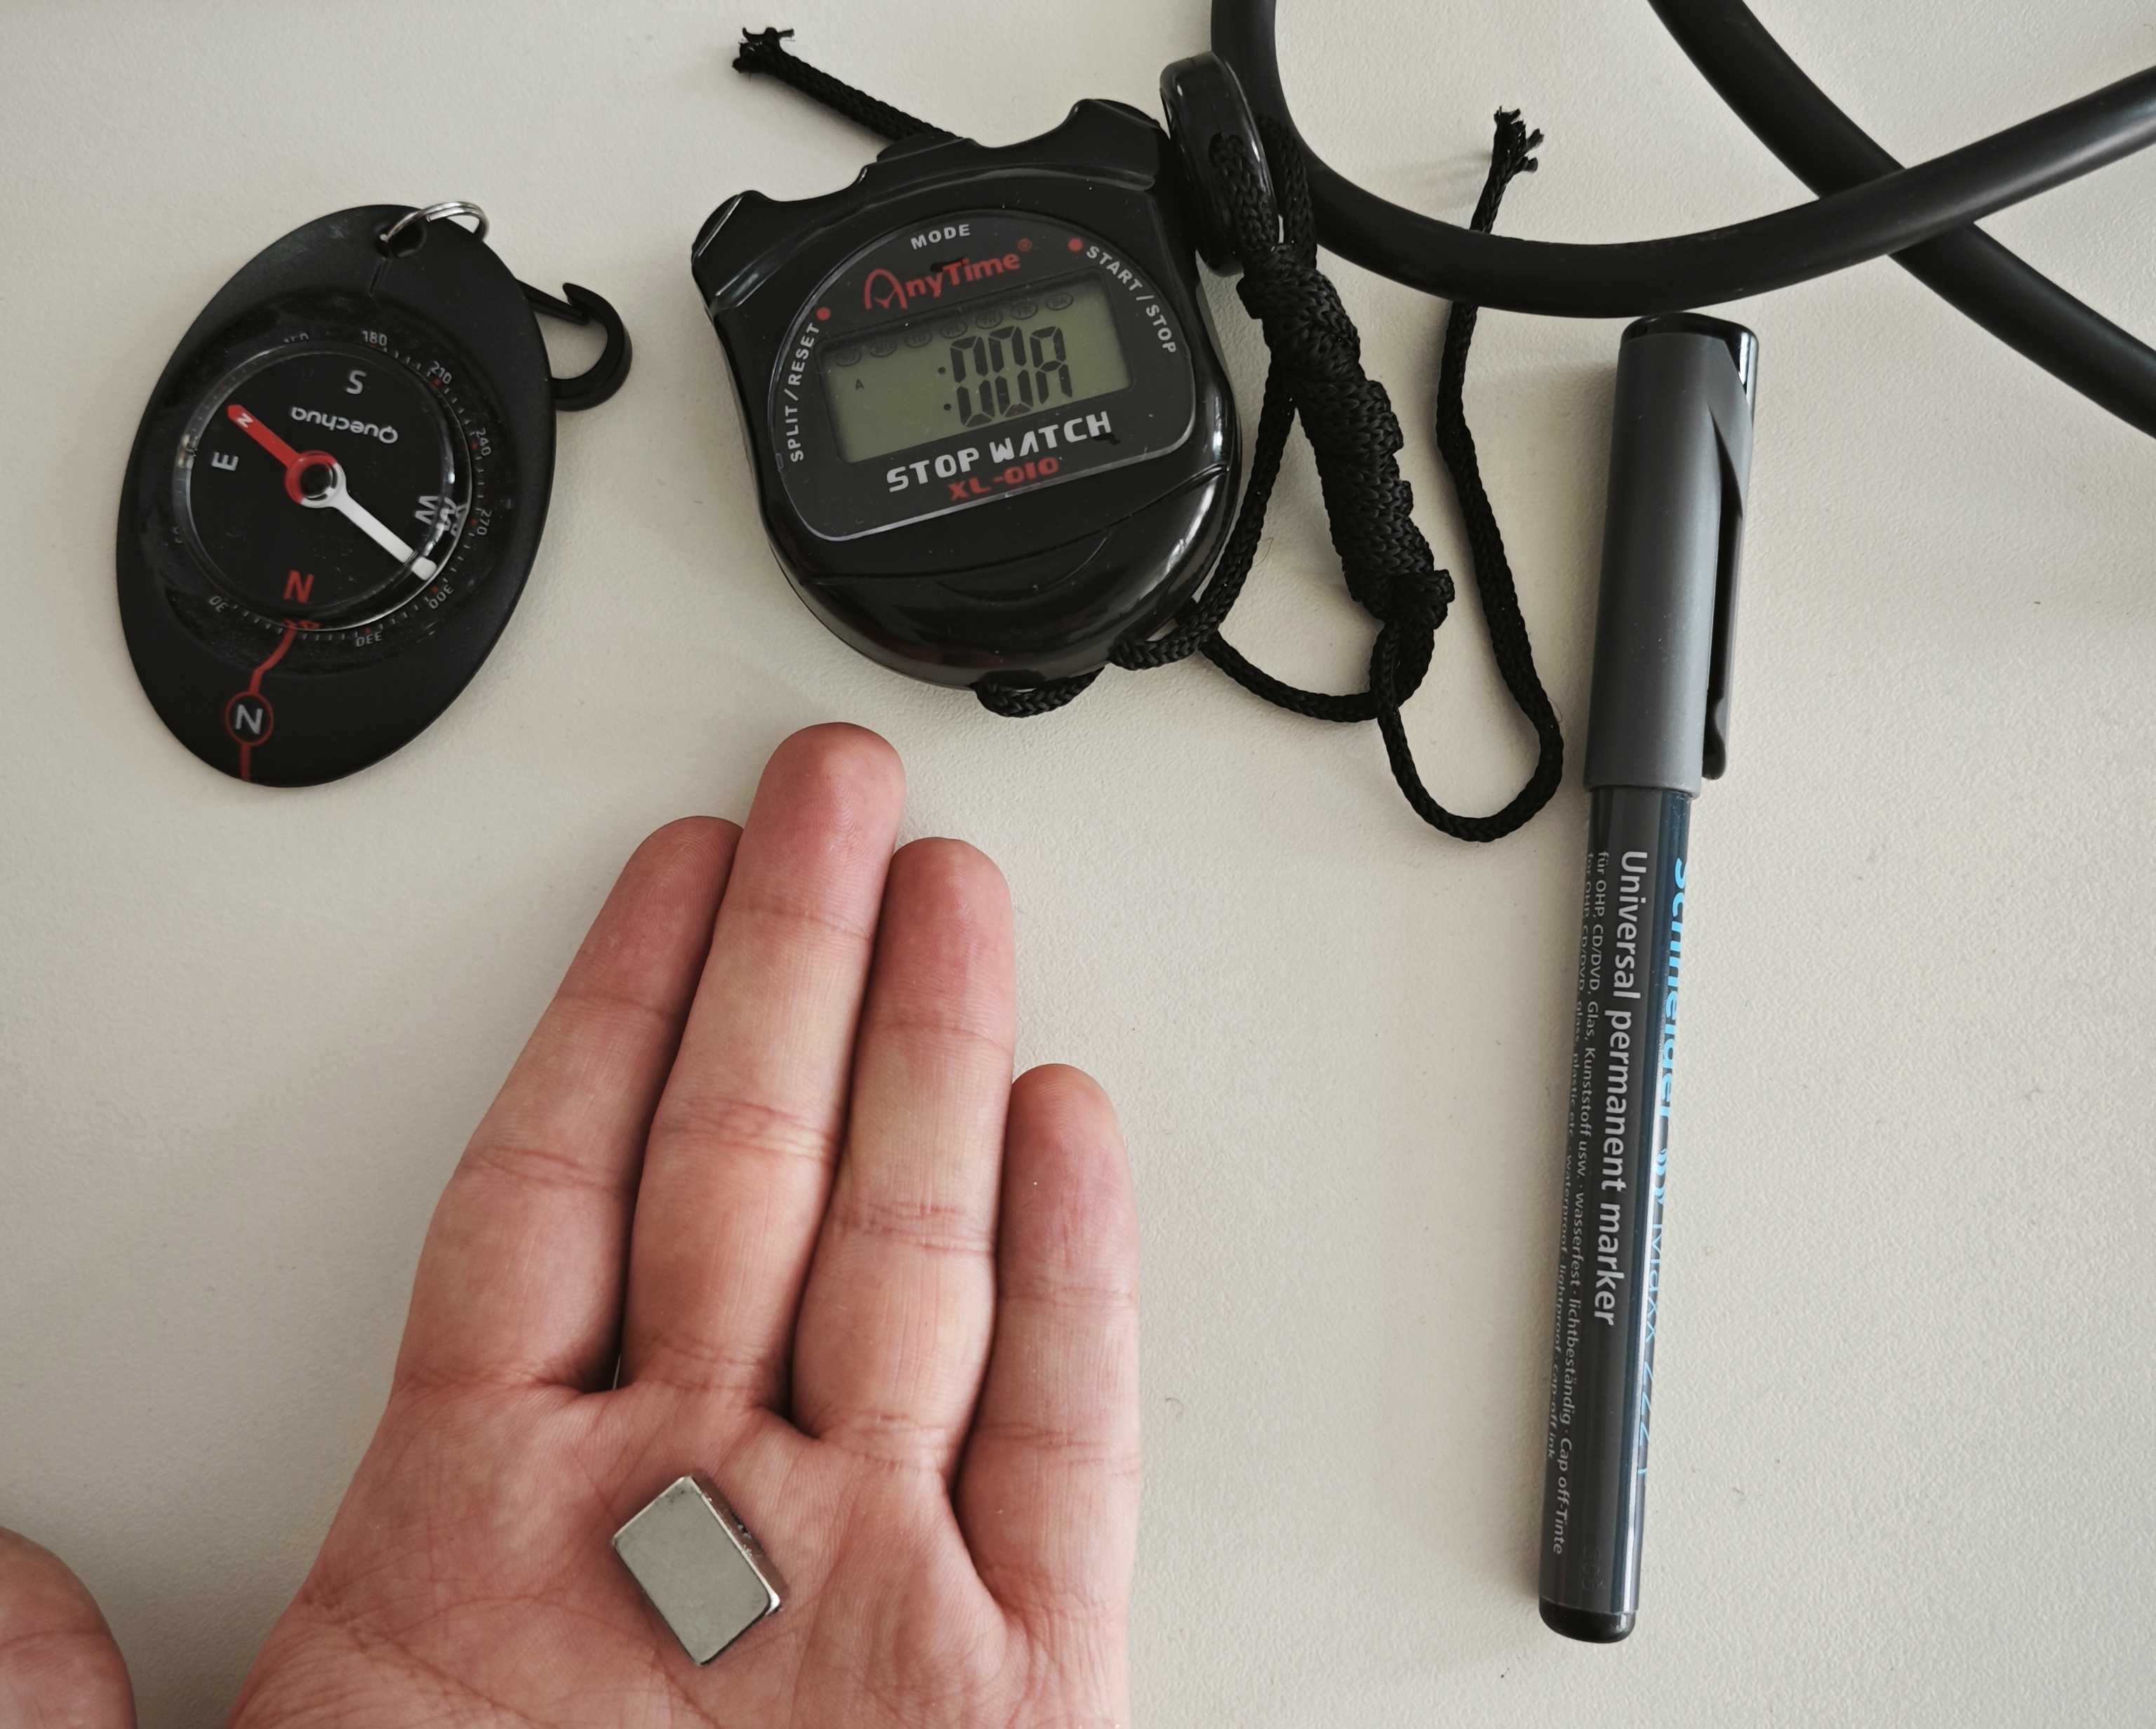
\includegraphics[width=0.40\textwidth]{fig/2017_e11.jpg}
\caption{Fingers.}
\label{fig1}
\end{figure}

The aim of this problem is to determine the horizontal component $B_0$ of the Earth's magnetic field, as well as the dipole moment $p$ of the neodymium magnet.\\

\textit{Tasks:}
\begin{subpart}
	\item Design and describe an experiment that can be used to find whether the magnets are magnetised along $a$, $b$, or $c$. Also find the surfaces corresponding to the north pole (N) and the south pole (S) of the magnet. Use the marker to indicate them on the magnet using the letters N and S.
	\item Study the deviation of the compass from the north-south axis at different distances $r$ between the needle and the neodymium magnet. The distance is measured between the centres of the objects. Using the data, plot a graph in the appropriate variables and use it to find the ratio $p/B_0$. Estimate your error.
	\item Design and carry out an experiment from which you can determine the product $pB_0$. Estimate your error. 
	\item Calculate the horizontal component of the Earth's magnetic field $B_0$ and the dipole moment $p$ of the magnet. Estimate your errors. 
\end{subpart}
\textbf{Note:} Do not falsify your data so as to obtain the textbook value of $B_0$. You will be in for a nasty surprise!\\

\textit{Relevant theory:}\\
1) A magnetic dipole moment $\mathbf{p}$ can be ascribed to any current $I$ circulating on a closed loop of surface $S$: 
\begin{equation*}
\mathbf{p}=IS \mathbf{n}
,
\end{equation*}
where $\mathbf{n}$ is a unit vector normal to the surface $S$. The units for dipole moment are [$\unit{A.m^2}$]. The atoms in permanent magnets can be treated as tiny current loops, meaning that permanent magnents also possess a net dipole moment. It points from their south pole to their north pole.\\

2) The point dipole approximation holds when the distance to a dipole $r$ is much larger than its characteristic length. Then the field along the axis of a dipole is given by
\begin{equation*}
\mathbf{B}=\frac{\mu_0\mathbf{p}}{2\pi r^3}
.
\end{equation*}
\begin{center}
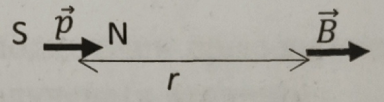
\includegraphics[width=0.3\textwidth]{fig/2017_e12.png}
\end{center}

3) When a dipole is placed in an external magnetic field $\mathbf{B_\mathrm{ext}}$, it experiences a torque
\begin{equation*}
	\mathbf{M}=\mathbf{p}\times\mathbf{B_\mathrm{ext}} \quad\quad (\mathrm{i.e.\,of\,magnitude}\,M=pB_\mathrm{ext}\sin{\theta})
.
\end{equation*}
that tends to rotate it towards the direction of the field.\\

4) The moments of inertia of a uniform rectangular cuboid about axes passing through its centre parallel to the edges $a$, $b$, and $c$, are respectively given by
\begin{equation*}
I_a=\frac{1}{12}m(b^2+c^2); \quad I_b=\frac{1}{12}m(c^2+a^2); \quad I_c=\frac{1}{12}m(a^2+b^2)
.
\end{equation*}
\end{eproblem}
\vspace{3ex}
\end{document}
